\clearpage
\section{Archived Strong-Baseline Architecture}\label{app:historical-design}
The following three diagrams preserve earlier system and research designs. Their dates, branch scope, and embedded labels are retained. The current evaluated method is the authorization pipeline in Figure~\ref{fig:architecture}.
\begin{center}
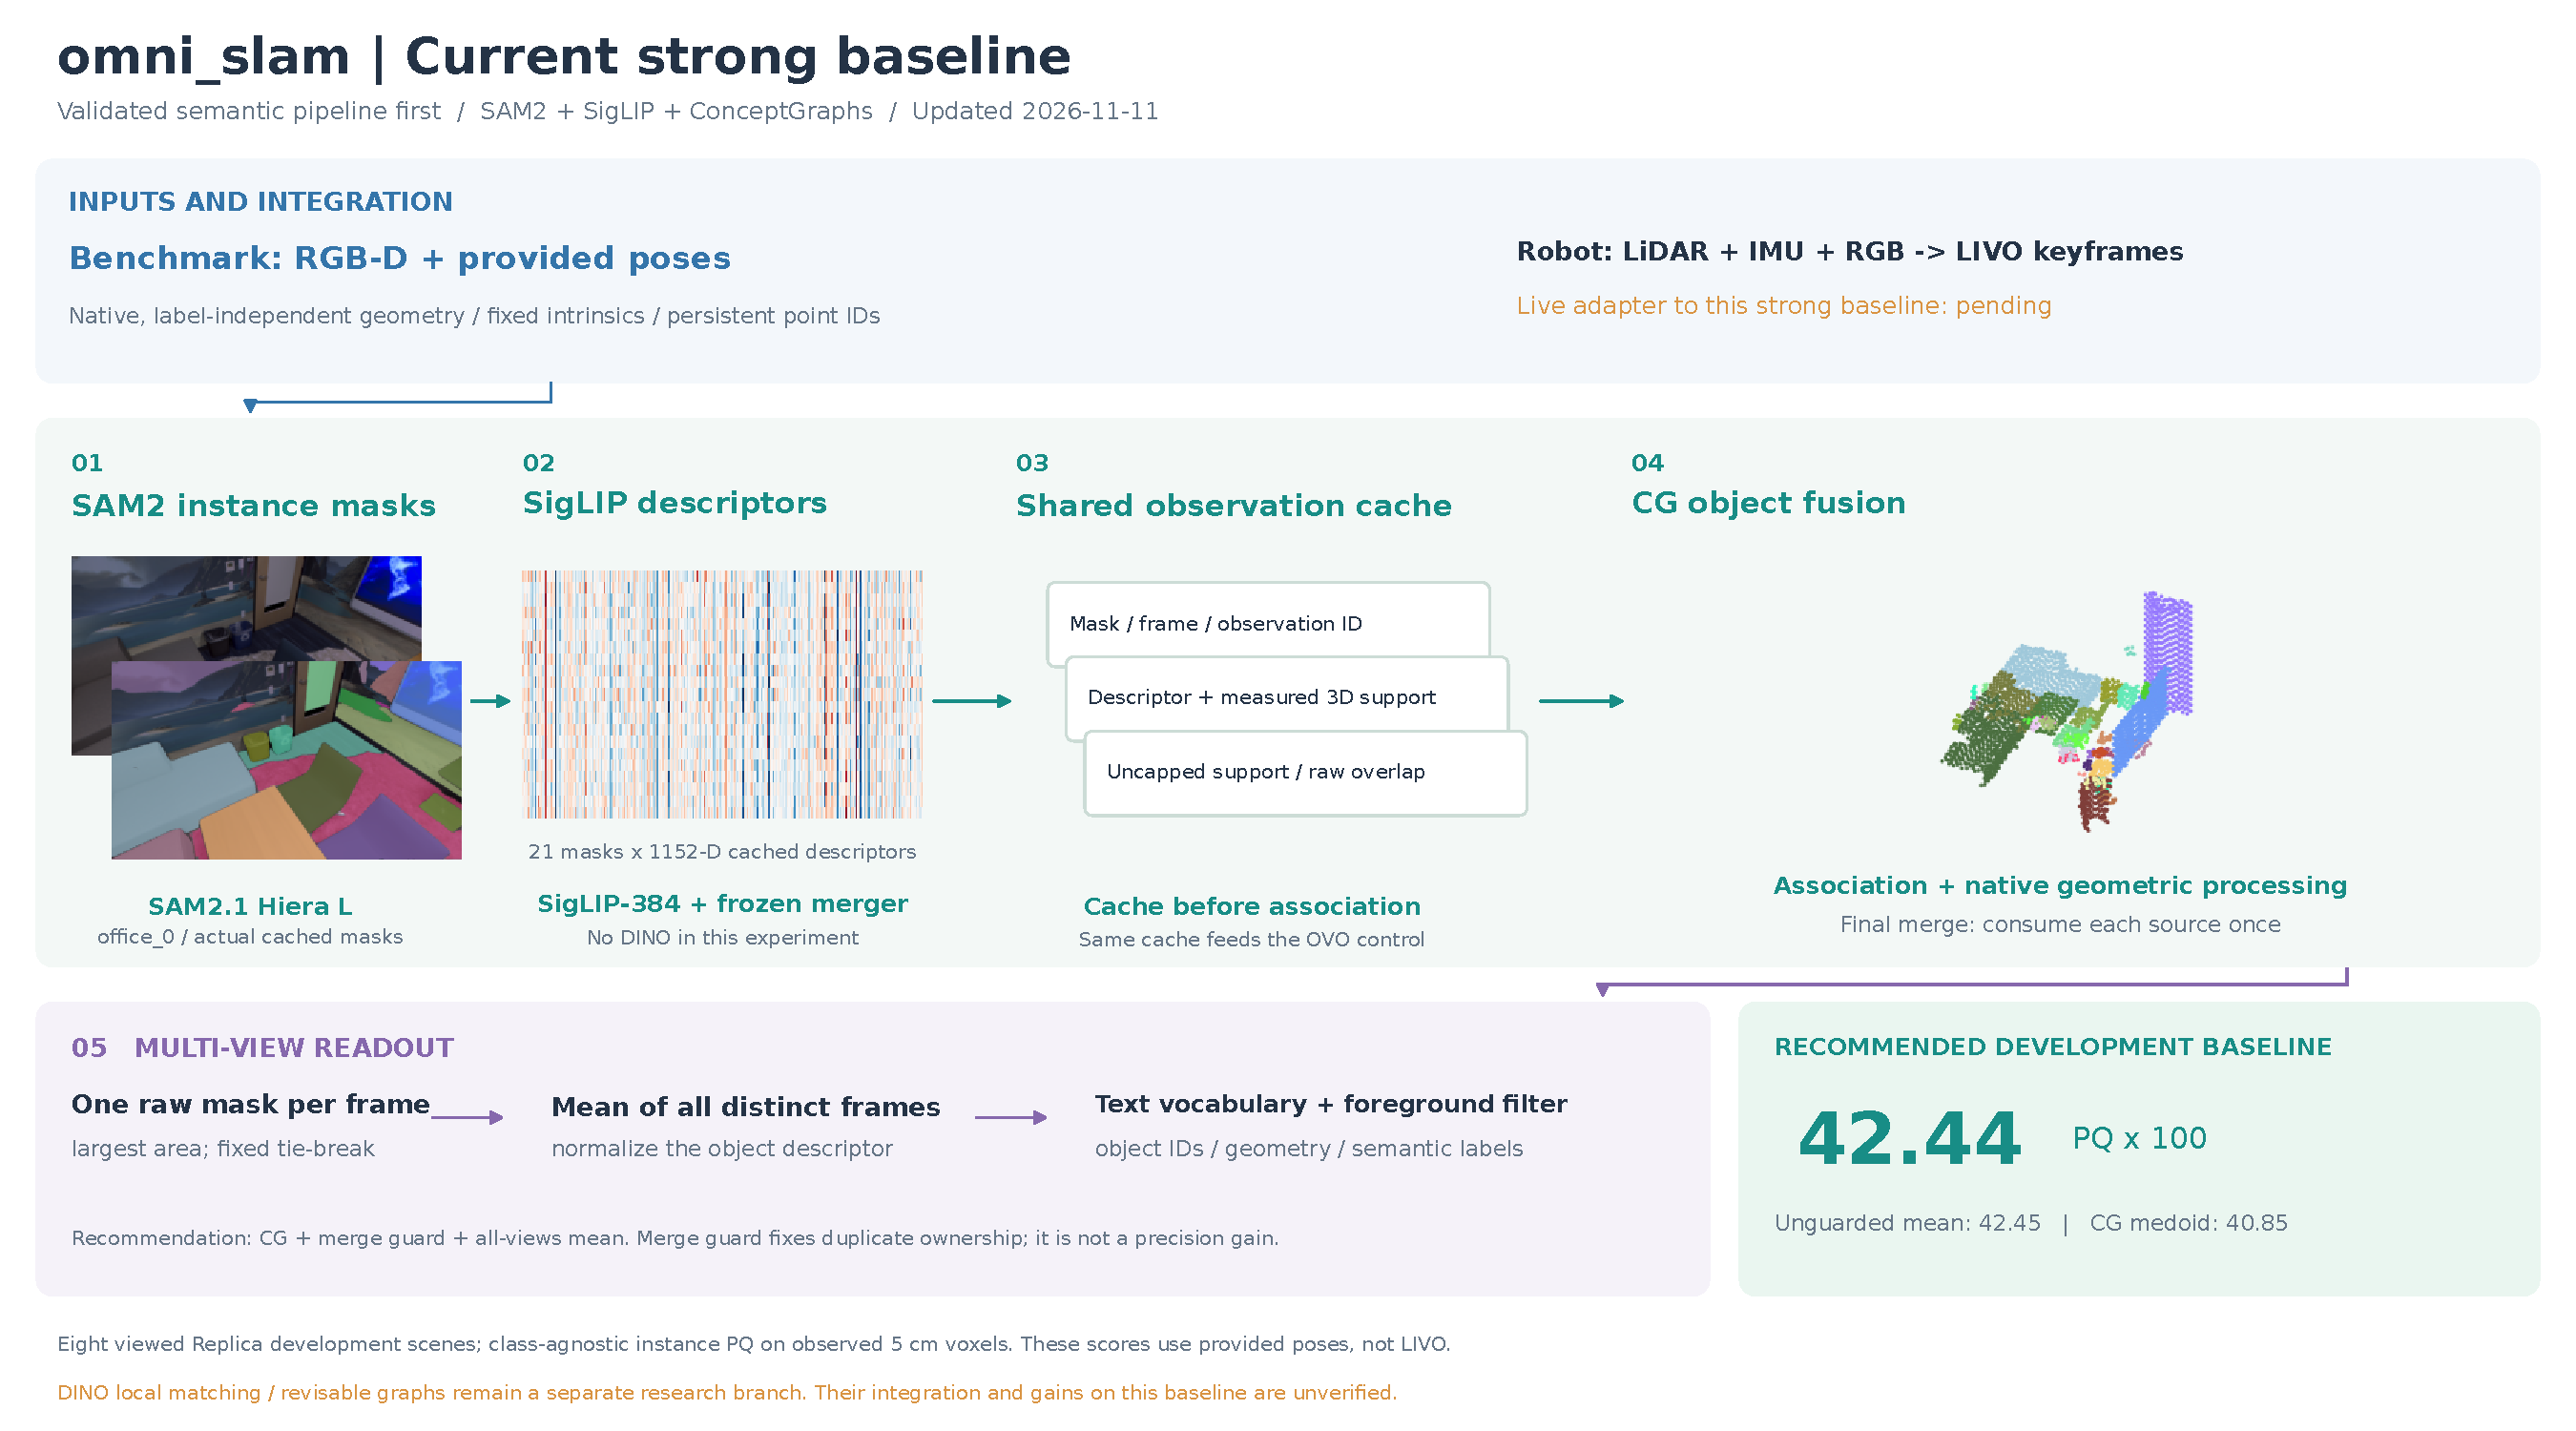
\includegraphics[width=\textwidth]{figures/history/omni_slam_current_baseline.pdf}
\captionof{figure}{Strong-baseline diagram from 11 November 2026. SAM2 and frozen SigLIP produce shared observations for ConceptGraphs-style fusion, a source-consumption guard, and a unique-frame mean semantic readout. The embedded title ``Current strong baseline'' refers to that dated revision. The 42.44 PQ value is from eight already-viewed Replica development scenes under its own observed 5\,cm domain; it is not current authorization performance.}
\end{center}
\subsection{What this diagram preserves}
The figure records the shared frontend, geometric fusion, and semantic readout before the later revision studies. Its robot adapter and DINO enhancement markers are design status from that revision. Current outdoor evaluation uses the separately documented SAM3-based branch; scores from these versions must not be pooled.

\clearpage
\section{Archived DINO--LIVO System Design}
\begin{center}
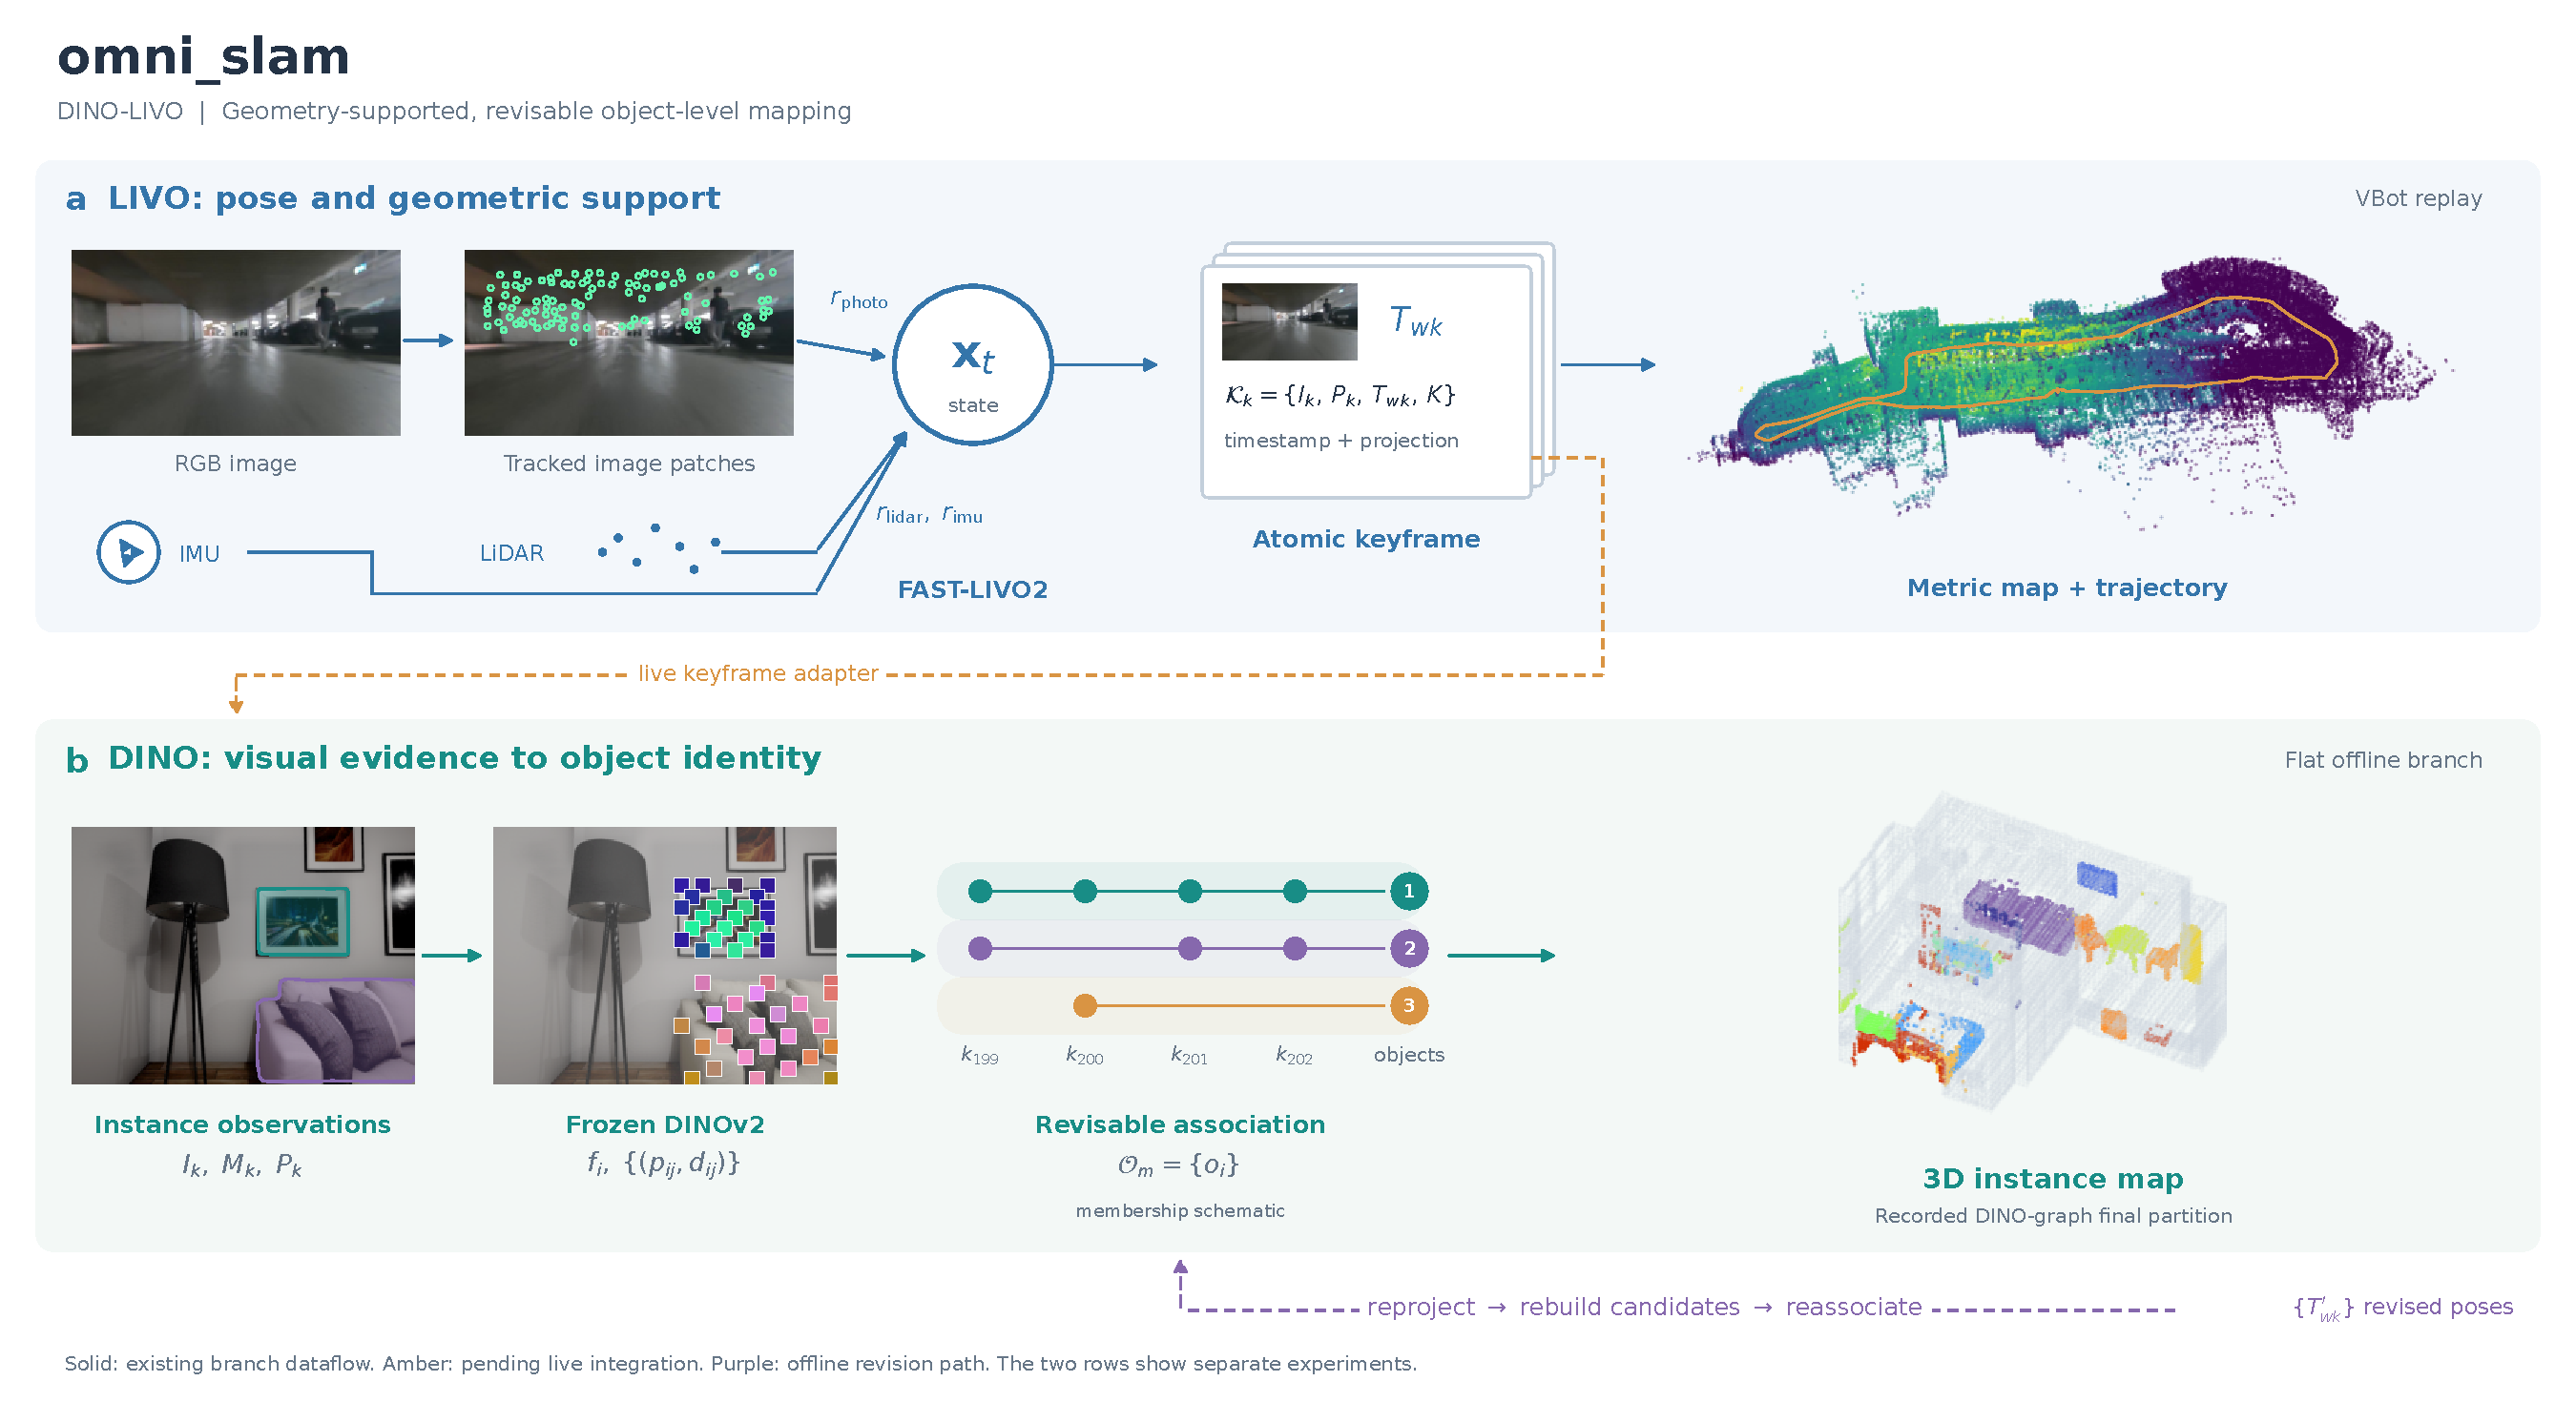
\includegraphics[width=\textwidth]{figures/history/dino_livo_system_architecture.pdf}
\captionof{figure}{DINO--LIVO design from 10 November 2026. The upper panel uses real VBot LIVO replay, while the lower panel uses a separate Flat offline DINO experiment. LIVO exports measured geometry and keyframes; frozen DINOv2 descriptors support an observation graph. The amber dashed connector denotes proposed live integration. This is not a jointly evaluated end-to-end system or the architecture used to obtain current outdoor AP.}
\end{center}
\subsection{Sensor and semantic interfaces}
The design retains the intended interface from image, LiDAR, and inertial processing to object observations and persistent identities. The two panels use different experiments and do not imply a shared trajectory or coordinate frame. DINOv2 feature extraction is distinct from Grounding DINO detection in the archived outdoor landmarks.

The current paper evaluates object-map revision with a frozen backbone. This archived design explains the broader project context; it does not imply that DINO tokens modify LIVO residuals or that a new association Transformer has been trained.

\clearpage
\section{Archived DINO Object-Graph Detail}
\begin{center}
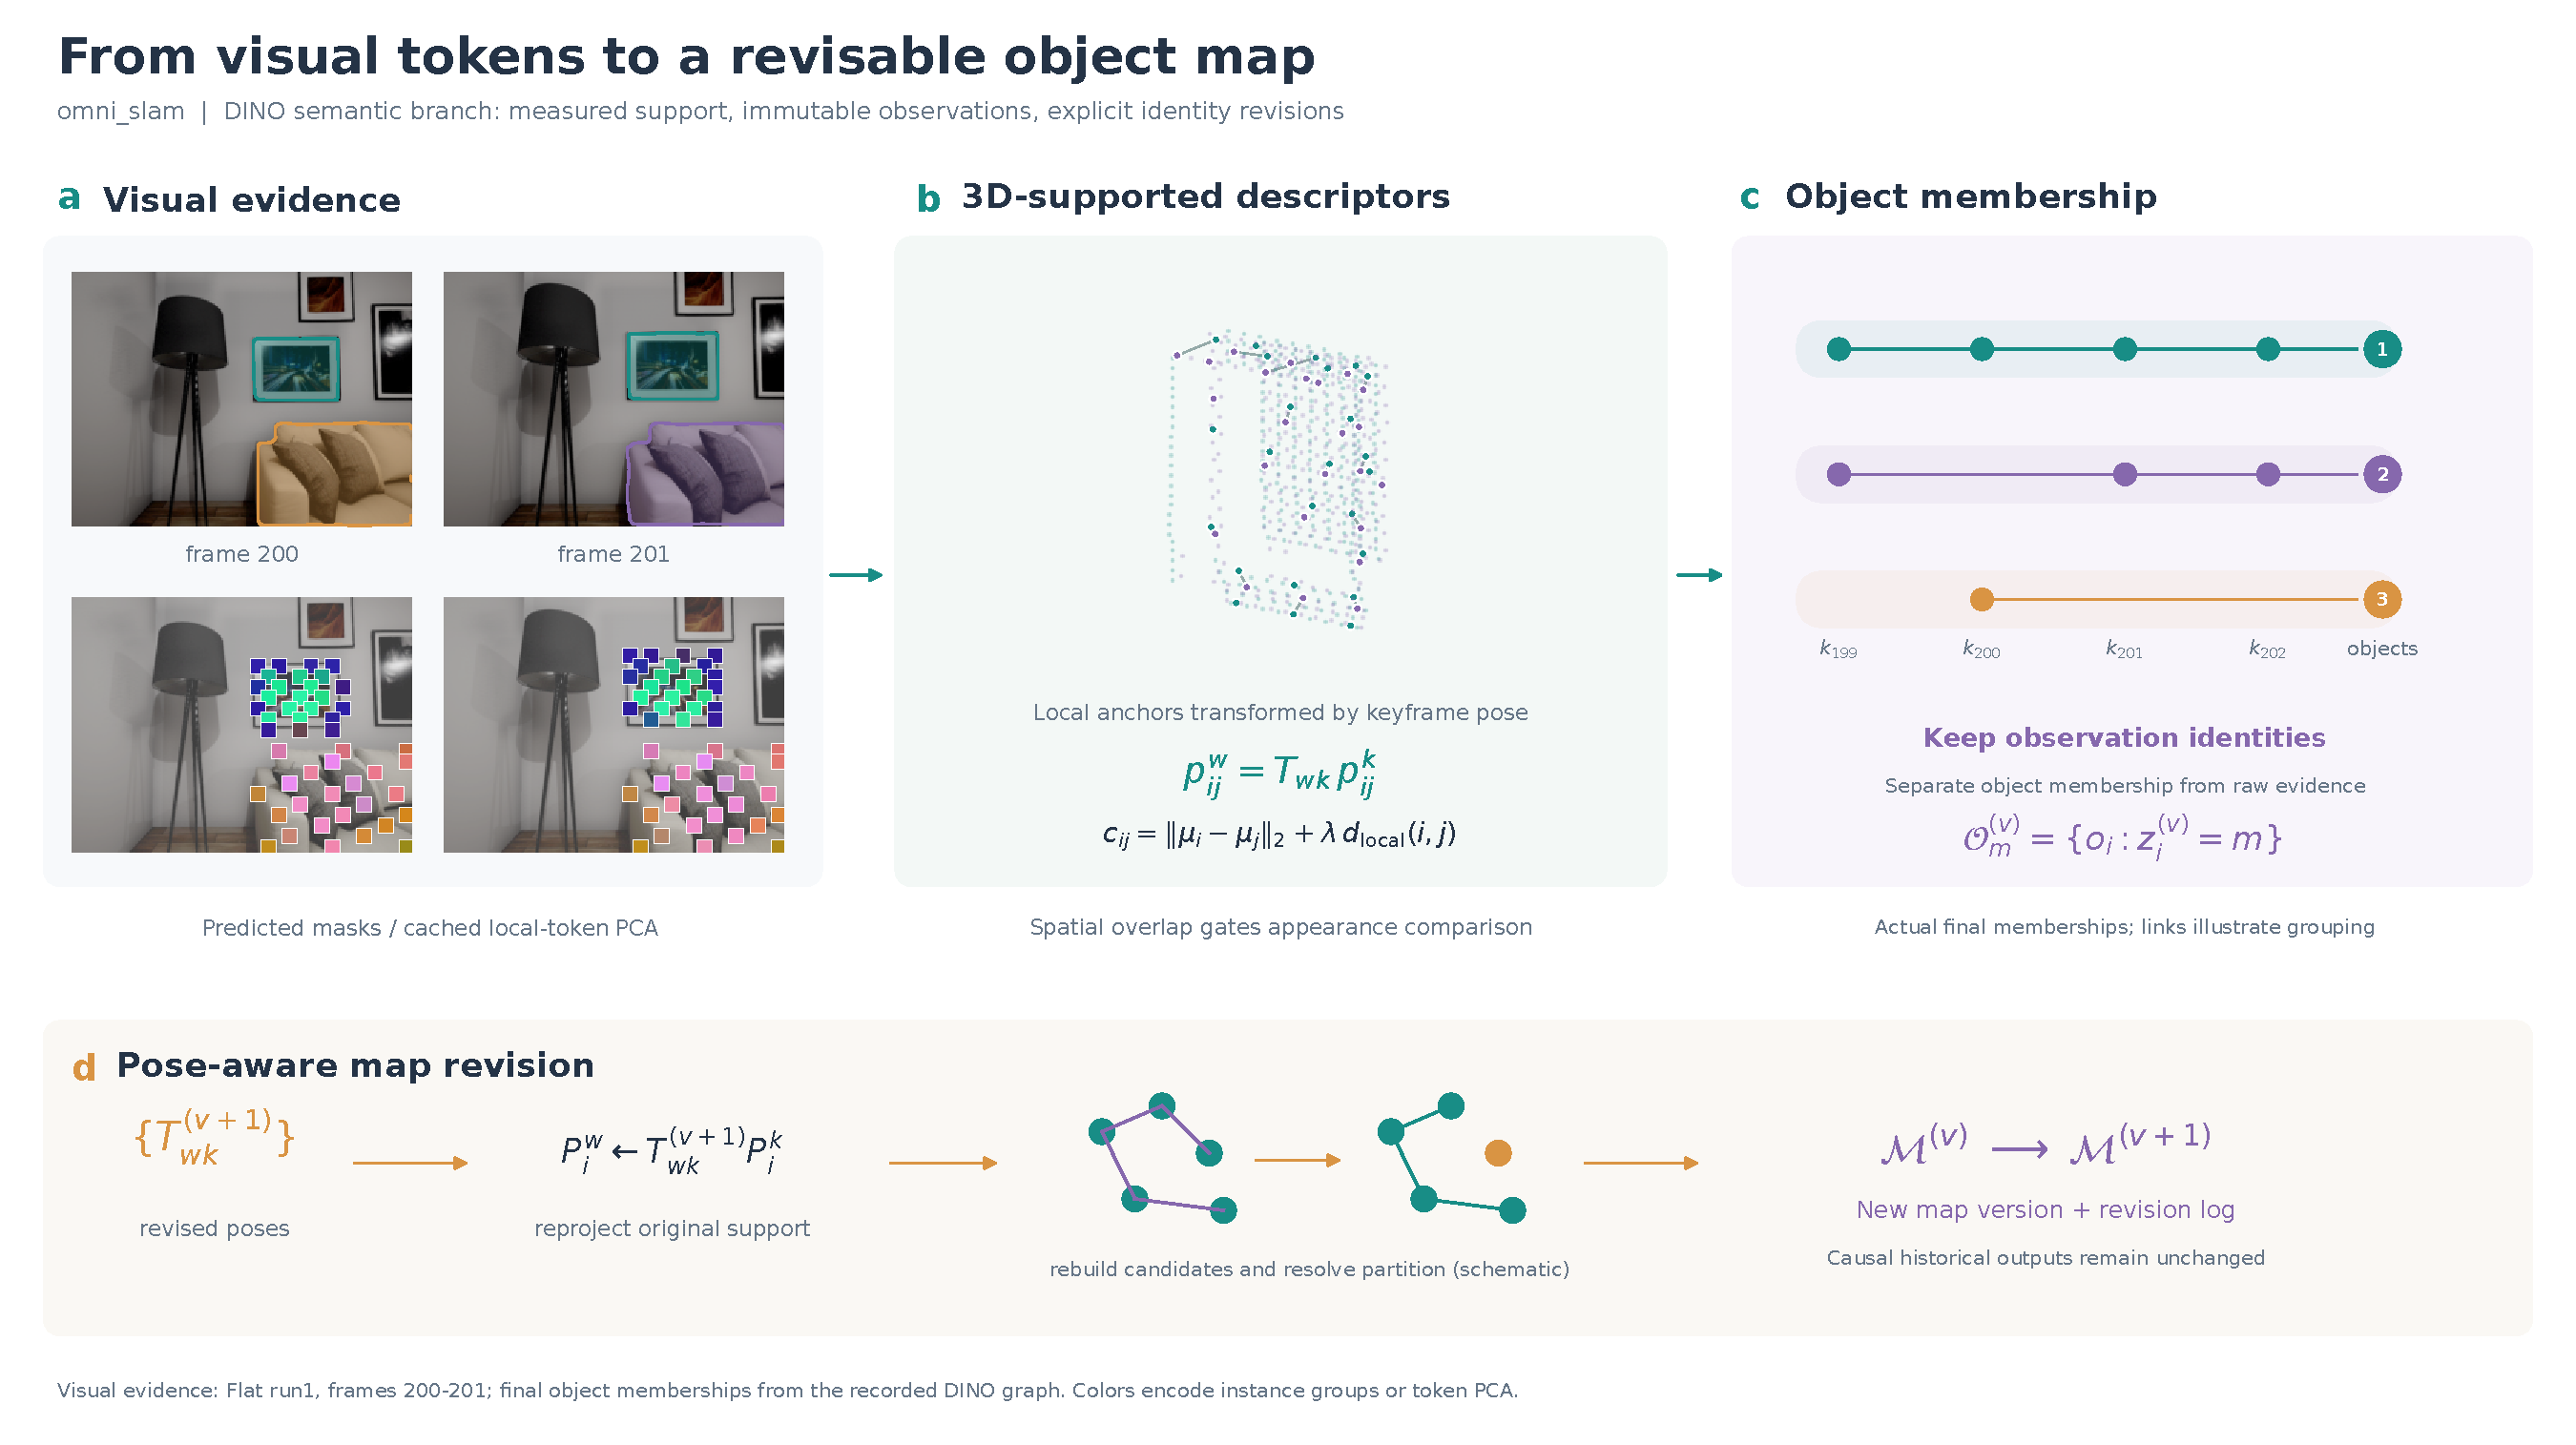
\includegraphics[width=\textwidth]{figures/history/dino_object_graph_detail.pdf}
\captionof{figure}{Geometry-supported DINO observations and map-revision design. Actual Flat run1 frames 200 and 201 supply masks and cached local descriptors, shown in one shared PCA basis. Measured depth anchors features in 3D; spatial support gates appearance comparison. Star links show recorded final memberships over frames 199--202, not original candidate edges. The pose-revision topology is schematic.}
\end{center}
\subsection{Interpretation of recorded memberships}
The displayed object numbers 1/2/3 correspond to original IDs 429/191/556. A sofa observation has different memberships across the selected frames; the original record is retained rather than presented as a repaired success. Feature colors are PCA visualizations, not semantic classes, attention weights, or matching confidence.

The diagram preserves an earlier candidate mechanism. It is neither an ablation of the current authorization rule nor evidence of stable DINO gains. The original input manifests are included with the three diagrams under \texttt{figures/history/}.
